\documentclass{beamer} 

\usepackage{hayesmacros}

\usetheme{metropolis}
\setsansfont{Fira Sans}  % be sure to compile with XeLaTeX

\usepackage{natbib}
\usepackage{ulem}
\usepackage{fontawesome5}

\newtheorem{proposition}{Proposition}
\newtheorem{assumption}{Assumption}

\theoremstyle{remark}
\newtheorem*{remark}{Remark}

\setbeamercolor{background canvas}{bg=white}
\setbeamercolor{normal text}{fg=black}
\setbeamercolor{frametitle}{bg=black, fg=white}

\hypersetup{colorlinks,citecolor=cyan, urlcolor=cyan, linkcolor=black}

\title{Estimating network-mediated causal effects via spectral embeddings}
\date{2022-10-14}
\author{Alex Hayes}
\institute{University of Wisconsin-Madison}


\begin{document}

\maketitle


\begin{frame}{This is joint work}
    \begin{columns}

        \column{0.49 \textwidth}

        \begin{figure}
            \includegraphics[width=0.8\textwidth]{figures/keith.jpg}
            \caption{Keith Levin, assistant professor in statistics}
        \end{figure}

        \column{0.49 \textwidth}

        \begin{figure}
            \includegraphics[width=0.9\textwidth]{figures/mystery-person2.jpg}
            \caption{You, our new collaborator??}
        \end{figure}

    \end{columns}

\end{frame}

\begin{frame}{Motivating example}

    \begin{columns}

        \column{0.4 \textwidth}

        \textbf{Does access to additional spending money cause adolescents to smoke, drink, and get high more often?}

        \column{0.6 \textwidth}

        Data

        \begin{itemize}
            \item Social network of 129 adolescents in secondary school in Glasgow, measured in 1995
            \item Spending money available to each adolescent
            \item Smoking (tobacco \& marijuana) and drinking behaviors
            \item Many potential controls
        \end{itemize}

    \end{columns}

\end{frame}

\begin{frame}
    \centering
    \vspace{3mm}
    \begin{figure}
        \includegraphics[width=\textwidth]{figures/glasgow-degree.png}
    \end{figure}

\end{frame}

\begin{frame}
    \centering
    \vspace{3mm}
    \begin{figure}
        \includegraphics[width=\textwidth]{figures/glasgow-alcohol.png}
    \end{figure}
\end{frame}

\begin{frame}
    \centering
    \vspace{3mm}
    \begin{figure}
        \includegraphics[width=\textwidth]{figures/glasgow-friendgroups.png}
    \end{figure}
\end{frame}

\section{Models of community membership in networks}

\begin{frame}{Homophily via stochastic blockmodels (SBMs)}

    \begin{columns}
        \column{0.45\textwidth}

        \begin{figure}
            \includegraphics[width=\textwidth]{figures/assortative.png}
        \end{figure}

        \column{0.55\textwidth}

        $d$ ``blocks'' or communities

        $Z_{i \cdot} \in \set{0, 1}^d$ one-hot indicator of node $i$'s block

        \vspace{4mm}

        $Z$ is latent (i.e. unobserved)

        \vspace{4mm}

        $B \in [0, 1]^{d \times d}$ inter-block edge probabilities

        $\P[Z]{A_{ij} = 1} = Z_{i \cdot} B Z_{j \cdot}^T$

        \vspace{4mm}

        Nodal outcomes $Y_i$, treatments $T_i$, and controls $C_i$ related to latent $Z$

    \end{columns}

\end{frame}

\begin{frame}{Stochastic blockmodels are good for intuition}

    ...but they do not encode a rich notion of homophily. SBMs can be extended:

    \begin{itemize}
        \item Differing node popularity
        \item Membership in multiple groups
        \item Partial memberships in groups
        \item Membership in multiple groups with group-specific popularity
        \item Etc, etc
    \end{itemize}

    All of these extensions can be captured in a more general model

\end{frame}

\begin{frame}{Sub-gamma random dot product graphs}

    \begin{definition}

        Let $A \in \R^{n \times n}$ be a random symmetric matrix, such as the adjacency matrix of an undirected graph. Let $\E[\X]{A} = \X \X^T$ be the expectation of $A$ conditional on $\X \in \R^{n \times d}$, which has independent and identically distributed rows $\X_{1 \cdot}, \dots, \X_{n \cdot}$. Conditional on $\X$, the elements of the upper triangle of $A - \E[\X]{A}$ are $(\nu_n, b_n)$-subgamma random variables.

    \end{definition}

    \textbf{Intuition}: the \emph{latent positions} $\X$ are very rich measures of community membership and node identity that live in $\R^d$

\end{frame}

\begin{frame}{Sub-gamma random dot product graphs}

    \begin{remark}
        We consider symmetric positive semi-definite $\E[\X]{A}$ to simplify notation, but everything works for generic $\E[\X]{A}$.
    \end{remark}

    \begin{remark}
        $\X$ is only identifiable up to orthogonal transformation, since $\E[\X]{A} = \X \X^T = (\X Q) (\X Q)^T$ for any $d \times d$ orthogonal matrix $Q$.
    \end{remark}

\end{frame}

\begin{frame}{Estimation via the adjacency spectral embedding}


    \begin{definition}[ASE]

        Given a network $A$, the $\widehat{d}$-dimensional \emph{adjacency spectral embedding} of $A$ is

        \begin{align*}
            \Xhat = \Uhat \Shat^{1/2}
        \end{align*}

        \noindent where $\Uhat \Shat \Uhat^T$ is the rank-$\widehat{d}$ truncated singular value decomposition of $A$.

    \end{definition}

    These are the ``principle components'' of the network

    The analyst must specify $\widehat{d}$

\end{frame}

\begin{frame}{Uniform consistency of the adjacency spectral embedding}

    \begin{lemma}[\cite{levin_recovering_2022}]

        Under the sub-gamma random dot product model and some additional omitted conditions, if $\widehat{d} = d$, there is some $d \times d$ orthogonal matrix $Q$ such that

        \begin{equation*}
            \max_{i \in [n]} \, \norm*{\Xhat_{i \cdot} - \X_{i \cdot} Q} = \op{1}.
        \end{equation*}

    \end{lemma}

\end{frame}

\section{Causal inference on networks}

\begin{frame}{Notation}
    \begin{columns}
        \column{0.45\textwidth}

        \begin{figure}
            \includegraphics[width=\textwidth]{figures/assortative.png}
        \end{figure}

        \column{0.55\textwidth}

        Network $A \in \R^{n \times n}$

        Nodal covariates $\W_{1 \cdot}, ..., \W_{n \cdot} \in \R^{p}$

        Latent positions $\X_{1 \cdot}, ..., \X_{n \cdot} \in \R^d$

        Nodal outcomes $Y_1, ..., Y_n \in \R$

        \vspace{6mm}

        Partition $\W_i = (T_i, \C_{i \cdot})$

        Treatment $T_i \in \set{0, 1}$

        Controls $\C_{i \cdot} \in \R^{p - 1}$

    \end{columns}
\end{frame}

\begin{frame}{The big picture}

    Homophily is a big deal when you're trying to do causal inference on a network.

    \cite{christakis_spread_2007} claimed obesity was socially contagious, to much fanfare. Statisticians have spent the subsequent 15 years curb-stomping the paper.

    Homophily can act as a \emph{powerful} confounder \citep{shalizi_homophily_2011}.

\end{frame}


\begin{frame}{Community membership can be a confounder}

    \begin{figure}
        \centering
        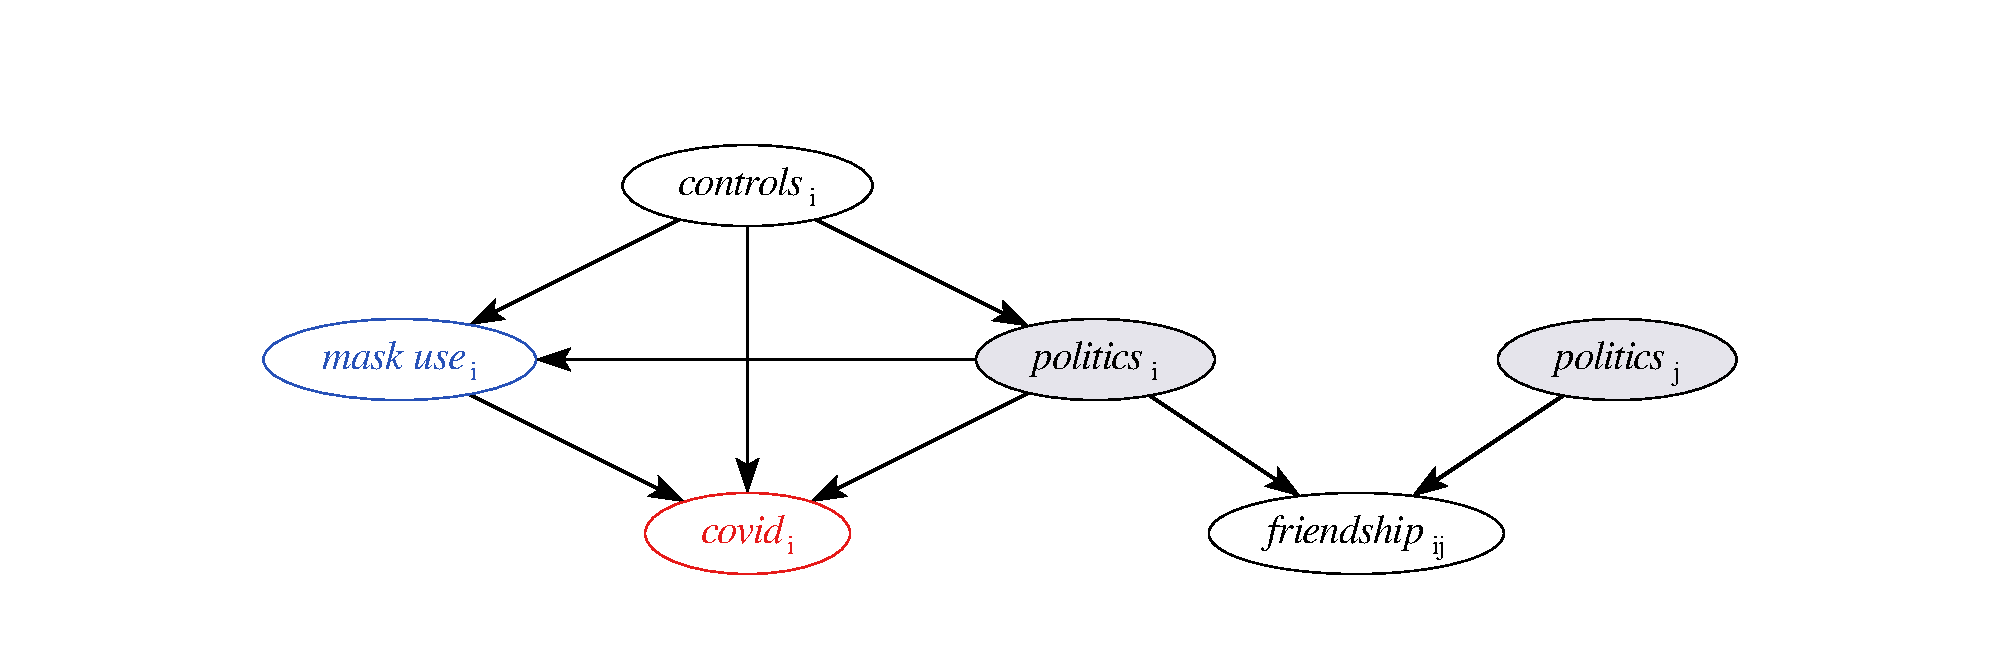
\includegraphics[width=1.1\textwidth]{figures/concrete-confounding-homophily.pdf}
        \caption{Directed acyclic graph (DAG) for node $i$. Portions of the DAG corresponding to nodes $j \neq i$ are omitted. $\X_i$ and $\X_j$ are not observed.}
        \label{fig:concrete-confounding}
    \end{figure}

\end{frame}

\begin{frame}{Community membership can be a mediator}

    \begin{figure}
        \centering
        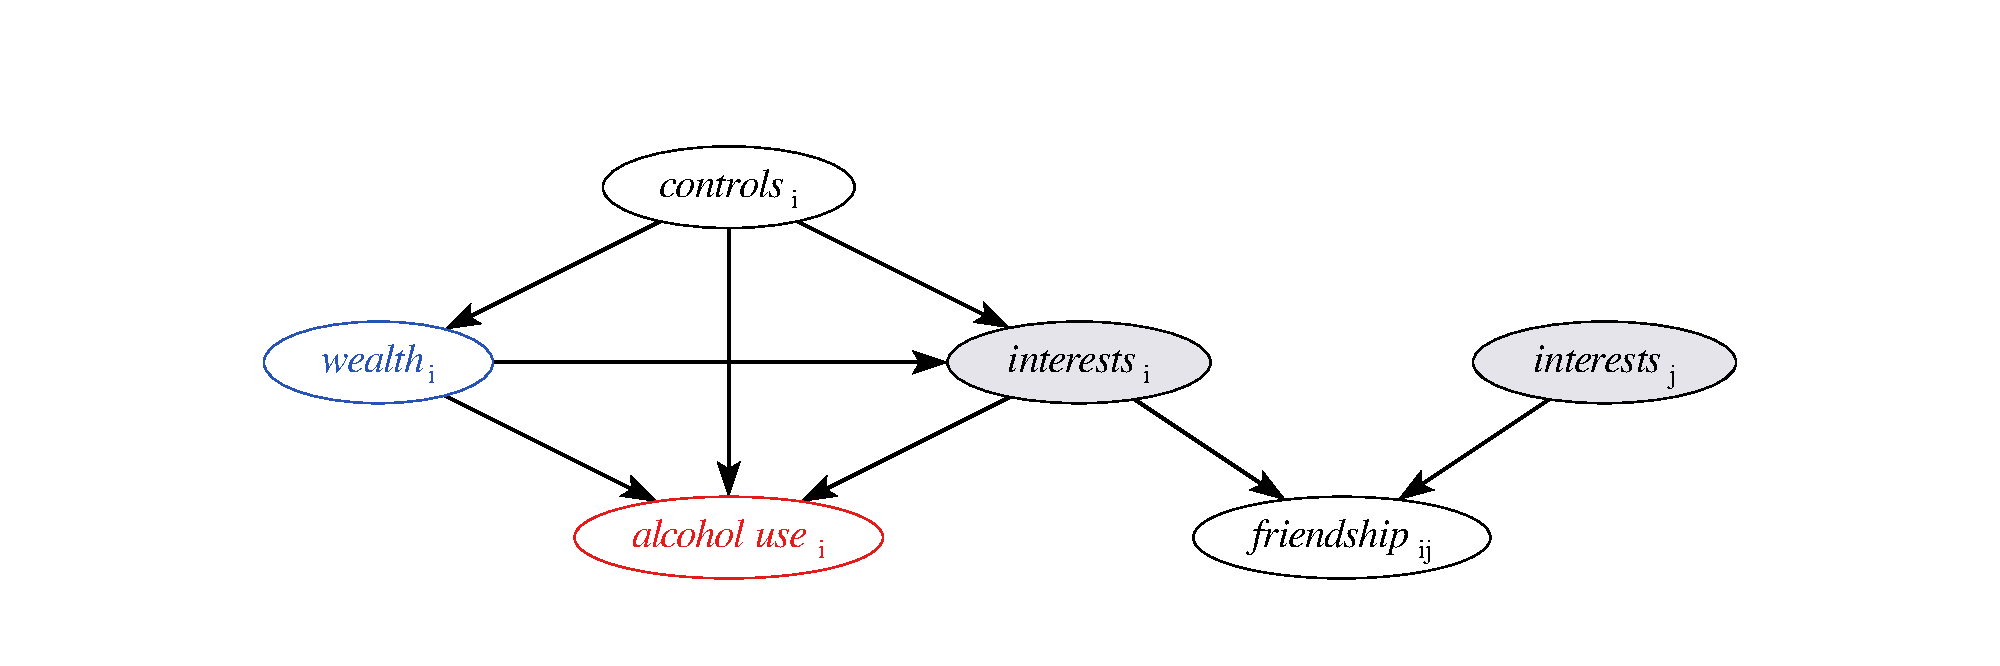
\includegraphics[width=1.1\textwidth]{figures/concrete-mediating-homophily.pdf}
        \caption{Directed acyclic graph (DAG) for node $i$. Portions of the DAG corresponding to nodes $j \neq i$ are omitted. $\X_i$ and $\X_j$ are not observed.}
        \label{fig:concrete-mediating}
    \end{figure}

\end{frame}

\begin{frame}{Causation and homophily}

    \textbf{Confounding homophily} is a big deal \citep{shalizi_homophily_2011}, and dealing with confounding homophily is a very active area of research.

    \vspace{3mm}

    \textbf{Mediating homophily} is somehow flying under the radar.
\end{frame}

\begin{frame}{Causal assumptions}

    \centering

    \begin{figure}
        \includegraphics[width=0.9\textwidth]{figures/mediating.png}
        \caption{Directed acyclic graph (DAG) for node $i$. Portions of the DAG corresponding to nodes $j \neq i$ are omitted. $\X_i$ and $\X_j$ are not observed.}
        \label{fig:mediating}
    \end{figure}

\end{frame}

\begin{frame}{Causal estimands}

    \begin{itemize}
        \item \emph{Average treatment effect}: how much the outcome $Y$ would change on average if the treatment $T$ were changed from $T = t$ to $T = t^*$

              \begin{equation*}
                  \ate = \E{Y_t - Y_{t^*}}
              \end{equation*}

        \item \emph{Controlled direct effect}: how much the outcome $Y$ would change on average if the mediator $\X$ were fixed at level $x$ uniformly in the population, but the treatment were changed from $T = t$ to $T = t^*$

              \begin{equation*}
                  \cde = \E{Y_{t \, x} - Y_{t^* \, x}}
              \end{equation*}

    \end{itemize}

\end{frame}

\begin{frame}{Causal estimands}

    \textbf{Warning:} slight change in notation. Now we consider a single node, and let $Y_{t x}$ denote a counterfactual.

    \begin{itemize}
        \item \emph{Natural direct effect}: how much the outcome $Y$ would change if the exposure $T$ were set at level $T = t^*$ versus $T = t$ but for each individual the mediator $\X$ were kept at the level it would have taken, for that individual, if $T$ had been set to $t^*$

              \begin{equation*}
                  \nde = \E{Y_{t \, \X_{t^*}} - Y_{t^* \, \X_{t^*}}}
              \end{equation*}

        \item Captures the effect of the exposure on the outcome that would remain if we were to disable the pathway from the exposure to the mediator

    \end{itemize}

\end{frame}

\begin{frame}{Causal estimands}

    \begin{itemize}
        \item \emph{Natural indirect effect}: how much the outcome $Y$ would change on average if the exposure were fixed at level $T = t^*$ but the mediator $\X$ were changed from the level it would take if $T=t$ to the level it would take if $T = t^*$

              \begin{equation*}
                  \nie = \E{Y_{t \, \X_{t}} - Y_{t \, \X_{t^*}}}
              \end{equation*}

        \item Captures the effect of the exposure on the outcome that operates by changing the mediator
    \end{itemize}

    \begin{equation*}
        \ate = \nde + \nie
    \end{equation*}

\end{frame}

\begin{frame}{Regression incorporating network principal components}

    Regression with rank-$\widehat{d}$ truncated singular value decomposition of $A$

    \begin{align*}
        \E[\X]{A}                           & = \X \X^T = \Upop \Spop \Upop^T             \\
        \E[\W_{i \cdot}, \X_{i \cdot}]{Y_i} & = \W_{i \cdot} \betaw + \X_{i \cdot} \betax
    \end{align*}

\end{frame}

\begin{frame}{Semi-parametric causal identification}

    If the mediation DAG holds (non-parametric assumption!) and additionally


    \begin{equation*} \begin{aligned}
            \underbrace{\E[T_i, \C_{i \cdot}, \X_{i \cdot}]{Y_i}}_{\R}
             & = \underbrace{\betazero}_{\R}
            + \underbrace{T_i}_{\{0, 1\}} \underbrace{\betat}_{\R}
            + \underbrace{\C_{i \cdot}}_{\R^{1 \times p'}} \underbrace{\betac}_{\R^{p'}}
            + \underbrace{\X_{i \cdot}}_{\R^{1 \times d}} \underbrace{\betax}_{\R^d}, \\
            \underbrace{\E[T_i, \C_{i \cdot}]{\X_{i \cdot}}}_{\R^{1 \times d}}
             & = \underbrace{\thetazero}_{\R^{1 \times d}}
            + \underbrace{T_i}_{\{0, 1\}} \underbrace{\thetat}_{\R^{1 \times d}}
            + \underbrace{\C_{i \cdot}}_{\R^{1 \times p'}} \underbrace{\Thetac}_{\R^{p' \times d}}
            + \underbrace{T_i}_{\{0, 1\}} \underbrace{\C_{i \cdot}}_{\R^{1 \times p'}} \underbrace{\Thetatc}_{\R^{p' \times d}}.
        \end{aligned} \end{equation*}

    Then:

    \begin{align*}
        \cdef & = \ndef = \paren*{t - t^*} \, \betat                                                \\
        \nief & = \paren*{t - t^*} \, \thetat \, \betax + (t - t^*) \, \mu_c \, \Thetatc \, \betax.
    \end{align*}

\end{frame}

\begin{frame}{Causal estimators}

    To estimate $\nde$ and $\nie$ in our semi-parametric setting, we combine regression coefficients from the network regression models:

    \begin{align*}
        \cdehat & = \ndehat = \paren*{t - t^*} \, \betathat                                                                              & \text{and} \\
        \niehat & = \paren*{t - t^*} \, \thetathat \, \betaxhat + \paren*{t - t^*} \cdot \widehat{\mu}_c \cdot \Thetatchat \, \betaxhat.
    \end{align*}

    It's standard to fit two regressions and multiply coefficients to estimate an indirect effect like this \citep{vanderweele_mediation_2014}.

\end{frame}


\begin{frame}{Our estimator: plug ASE into ordinary least squares}

    Let $\Dhat = \begin{bmatrix} \W & \Xhat \end{bmatrix} \in \mathbb{R}^{n \times (p + d)}$. We estimate $\betaw$ and $\betax$ via ordinary least squares as follows

    \begin{align*}
        \begin{bmatrix}
            \betawhat \\
            \betaxhat
        \end{bmatrix}
        = \paren*{\Dhat^T \Dhat}^{-1} \Dhat^T Y.
    \end{align*}

    Similarly, we estimate $\Theta$ via ordinary least squares as

    \begin{align*}
        \Thetahat
        = \paren*{\W^T \W}^{-1} \W^T \Xhat.
    \end{align*}
\end{frame}

\begin{frame}{Main statistical result}

    \begin{theorem}[Regression coefficients are asymptotically normal]

        \vspace{2mm}

        Under some mild assumptions

        \begin{equation*}
            \begin{aligned}
                \sqrt{ n } \,
                 & \Sigmahatbeta^{-1/2}
                \begin{pmatrix}
                    \betawhat - \betaw \\
                    Q \, \betaxhat - \betax
                \end{pmatrix}
                \to
                \Normal{0}{I_d}, and     \\
                \sqrt{ n } \,
                 & \Sigmahattheta^{-1/2}
                \begin{pmatrix}
                    \vecc \paren*{\Thetahat \, Q^T} - \Thetavec
                \end{pmatrix}
                \to
                \Normal{0}{I_{p d}}.
            \end{aligned}
        \end{equation*}

        \noindent where $\Sigmahattheta^{-1/2}$ and $\Sigmahatbeta^{-1/2}$ are the robust covariance estimators based on $(\Dhat, Y, \betahat)$ and $(\W, \Xhat, \Thetahat)$, respectively.
    \end{theorem}
\end{frame}

\begin{frame}{Main causal result}

    \begin{theorem}[Causal estimators are asymptotically normal]

        \vspace{2mm}

        Under the same statistical assumptions as before, plus mediating homophily,

        \begin{align*}
            \sqrt{n \, \sigmahatnde} \paren*{\ndehat - \nde}
             & \to
            \Normal{0}{1}, \text { and } \\
            \sqrt{n \, \sigmahatnie} \paren*{\niehat - \nie}
             & \to
            \Normal{0}{1}.
        \end{align*}

        \noindent where $\sigmahatnde$ and $\sigmahatnie$ are rather unfriendly variance estimators derived via the delta method and the previous theorem.

    \end{theorem}

\end{frame}

\begin{frame}{Application to Glasgow data}
    TODO
\end{frame}

\begin{frame}{Thank you! Questions?}

    \textbf{Follow-up work we're interested in}

    \begin{itemize}
        \item Better identifiability via varimax rotation
        \item Extension to GLMs
        \item Accommodating network interference
    \end{itemize}

    Contact me if you'd like to work on any of these!

    \begin{itemize}
        \item[] \faIcon{twitter} \href{https://twitter.com/alexpghayes}{@alexpghayes}
        \item[] \faIcon{inbox} \href{mailto:alex.hayes@wisc.edu}{alex.hayes@wisc.edu}
        \item[] \faIcon{dice-four} \url{https://www.alexpghayes.com}
    \end{itemize}

\end{frame}


% \begin{frame}{Choosing the rank of the network}

%     \begin{itemize}
%         \item Use cross-validated eigenvalues by \cite{chen_estimating_2021}
%         \item Check sensitivity of results to choice of $k$
%     \end{itemize}

%     \begin{figure}
%         \includegraphics[width=0.9\textwidth]{figures/presentation/rank.png}
%         \label{fig:rank}
%     \end{figure}

%     % Tianxi asks: is the rank estimate too high?
% \end{frame}


\section{Appendix}


\begin{frame}{Choosing the rank of the network}

    \begin{itemize}
        \item Use cross-validated eigenvalues by \cite{chen_estimating_2021}
        \item Check sensitivity of results to choice of $\widehat{d}$
    \end{itemize}

    TODO: rank misspecification figure goes here

\end{frame}

\begin{frame}{Identifying assumptions}

    We require that natural direct and indirect effects are identified, as follows from consistency, positivity, and sequential ignorability \citep{imai_identification_2010}.

    \begin{itemize}

        \item Consistency:

              \begin{equation*}
                  \begin{aligned}
                       & \text{if $T = t$, then $\X_t = X$ with probability 1, and}               \\
                       & \text{if $T = t$ and $\X = x$, then $Y_{t \, x} = Y$ with probability 1}
                  \end{aligned}
              \end{equation*}

        \item Positivity:

              \begin{equation*}
                  \begin{aligned}
                      \P[T, \C]{x} & > 0 \text{ for each }  x \in \supp(\X) \\
                      \P[\C]{t}    & > 0 \text{ for each }  t \in \supp(T)
                  \end{aligned}
              \end{equation*}

    \end{itemize}

\end{frame}

\begin{frame}{Identifying assumptions}

    \begin{itemize}

        \item Sequential ignorability:

              \begin{equation*}
                  \begin{aligned}
                      \set{Y_{t^* \, x}, \X_t} \indep T & \cond \C        \\
                      \set{Y_{t^* \, x}} \indep \X      & \cond T = t, \C
                  \end{aligned}
              \end{equation*}

    \end{itemize}

    This is a criminally strong assumption, in all honesty. Requires the mediator $\X$ to be unconfounded with the outcome $Y$.

\end{frame}


\begin{frame}{Interventions on a network}

    \begin{figure}
        \includegraphics[width=\textwidth]{figures/intervention.pdf}
        \caption{Canonical intervention when $\C$ is highly informative.}
        \label{fig:intervention}
    \end{figure}
\end{frame}

\begin{frame}{Interventions on a network}

    \begin{align*}
        \underbrace{\E[T_i, \C_{i \cdot}]{\X_{i \cdot}}}_{\R^{1 \times d}}
         & = \underbrace{\thetazero}_{\R^{1 \times d}}
        + \underbrace{T_i}_{\{0, 1\}} \underbrace{\thetat}_{\R^{1 \times d}}
        + \underbrace{\C_{i \cdot}}_{\R^{1 \times p'}} \underbrace{\Thetac}_{\R^{p' \times d}}
        + \underbrace{T_i}_{\{0, 1\}} \underbrace{\C_{i \cdot}}_{\R^{1 \times p'}} \underbrace{\Thetatc}_{\R^{p' \times d}}.
    \end{align*}

    In Figure \ref{fig:intervention}, $\C$ are latent parameters for a DC-SBM and $\thetazero = \vec 0, \thetat = \vec 0, \Thetac = I_k$ and

    \begin{align*}
        \Thetatc =
        \begin{bmatrix}
            -1 & 2 & 0  & 0 & 0 \\
            0  & 0 & 0  & 0 & 0 \\
            0  & 1 & -1 & 0 & 0 \\
            0  & 0 & 0  & 0 & 0 \\
            0  & 0 & 0  & 0 & 0 \\
        \end{bmatrix}
    \end{align*}
\end{frame}

\bibliographystyle{chicago}
\bibliography{references}

\end{document}